\documentclass[12pt, a4paper]{report}

% Импорты 

\usepackage{cmap}
\usepackage{url}
\usepackage{hyperref}
\usepackage{amsthm, amsmath, amssymb}
\usepackage{thmtools}
\usepackage{fancyhdr}
\usepackage{graphicx}
\usepackage{titlesec}
\usepackage[normalem]{ulem}

\usepackage[english, russian]{babel}
\usepackage[utf8]{inputenc}
\usepackage[T2A]{fontenc}

% Геометрия 

\usepackage{geometry}
\geometry{
	left=1.5cm,
	right=1.5cm,
	top=2cm,
	bottom=1.5cm
}

\setlength\parindent{0pt}

% Теоремы, леммы ...

\renewcommand{\listtheoremname}{Список теорем}

\newtheorem{theorem}{Теорема}[section]
\newtheorem{lemma}[theorem]{Лемма}
\newtheorem{corollary}[theorem]{Следствие}
\theoremstyle{definition}
\newtheorem*{definition}{Определение}
\theoremstyle{remark}
\newtheorem{remark}[theorem]{Замечание}
\newtheorem{example}[theorem]{Пример}
% Колонтитулы

\pagestyle{fancy}
\fancyhf{}
\fancyhead[R]{\rightmark}
\fancyhead[L]{\textsc{\thechapter. \leftmark}}
\fancyfoot[C]{\thepage}
\renewcommand{\chaptermark}[1]{\markboth{#1}{}}
\renewcommand{\sectionmark}[1]{\markright{#1}}

% Главы

\titleformat{\chapter}[display]
{\normalfont\huge\bfseries\centering} % Формат текста
{\titlerule[1pt] \vspace{1pt} \titlerule\vspace{1pc} \Huge\MakeUppercase{\chaptertitlename} \thechapter} % Номер главы
{1pc} % Отступ между номером главы и названием
{\Huge} % Формат названия главы
[\vspace{1pc} \titlerule] % Декоративные элементы после названия

\titlespacing*{\chapter}{0pt}{0pt}{40pt}

\begin{document}
	
	\begin{titlepage}
		\newgeometry{left=1.5cm, right=1.5cm, top=3cm, bottom=2cm}
		\centering
		
		{\Large Санкт-Петербургский губернаторский\\ Физико-математический лицей №30}\\[1cm]
		
\includegraphics[width=0.18\textwidth]{assets/logo.png}\\[5cm]
		
		\textbf{ \LARGE Конспект уроков алгебры 8-го класса}\\[2cm]
		
		\begin{flushright}
			\textbf{Ученика:} \\ Лавелина М.Е. \\[1cm]
			\textbf{По мотивам уроков:} \\ Ренёва О.В. \\[1cm]
		\end{flushright}
		
		\vfill
		
		{\large 2023--2024 г.}
		
	\end{titlepage}
	
	\begin{abstract}

		\textbf{\Large Конспект находится в разработке, он может быть неполный, содержать ошибки, и вообще, думайте своей головой.} \\[1.5cm]
	
		Как вы могли понять из названия, ниже будет представлен материал 8 класса Санкт-Петербургскго губернаторского лицея. 
		Я постарался максимально точно перенести содержание своего бумажного конспекта, надеюсь вам понравится. \\
		
		\begin{center}
		  Удачи в изучении алгебры!
		\end{center} 
		
	  \end{abstract}

	\newgeometry{left=1.5cm, right=1.5cm, top=1cm, bottom=2cm}
\tableofcontents
\setcounter{page}{0} 
\thispagestyle{empty}
\restoregeometry
	
	\chapter{Элементы математической логики}

\section{Основные определения}

\begin{definition}[Высказывание]
	Предложение на естественном языке об истинности или ложности которого можно однозначно судить.
\end{definition}

\begin{example}
	Луна -- спутник марса.
\end{example}

\begin{example}
	$2 + 3 = 5$
\end{example}

\begin{example}
	\uwave{100 -- очень большое число} $\leftarrow$ не высказывание, для кого-то большое, а для кого-то нет.
\end{example}

\begin{definition}[Предикат]
	Предложение, содержащие одну или несколько переменных, при замене которых на конкретные значения становится высказыванием.
\end{definition}

\begin{example}
	Меня зовут Маша.
\end{example}

\begin{example}
	$x + 3 = 5$
\end{example}

\section{Конъюнкция, дизъюнкция, отрицание}

\begin{definition}[Отрицание]
	Отрицанием высказывания $A$ называется высказывание, обозначаемое $\overline A$, $\neg A$ (произносится как <<не А>>), истинность которого определяется таблицей:
	\begin{center}
		\begin{tabular}{ |c|c| } 
			\hline
			$A$ & $\neg A$ \\
			\hline 
			1 & 0 \\ 
			0 & 1 \\ 
			\hline
		\end{tabular}
	\end{center}
\end{definition}

\begin{definition}[Конъюнкция]
	Конъюнкцией высказываний $A$ и $B$ называется высказывание, обозначаемое $A \land B$, $A \& B$, значок фигурных скобок между $A$ и $B$ (произносится как <<А и Б>>), истинность которого определяется таблицей:
	\begin{center}
		\begin{tabular}{ |c|c|c| } 
			\hline
			$A$ & $B$ & $A \land B$ \\
			\hline 
			1 & 1 & 1 \\ 
			1 & 0 & 0 \\
			0 & 1 & 0 \\ 
			0 & 0 & 0 \\  
			\hline
		\end{tabular}
	\end{center}
\end{definition}

\begin{definition}[Дизъюнкция]
	Дизъюнкцией высказываний  $A$ и $B$ называется высказывание, обозначаемое $A \lor B$, $\neg A$, значок квадратных скобок между $A$ и $B$(произносится как <<А или Б>>), истинность которого определяется таблицей:
	\begin{center}
		\begin{tabular}{ |c|c|c| } 
			\hline
			$A$ & $B$ & $A \lor B$ \\
			\hline 
			1 & 1 & 1 \\ 
			1 & 0 & 1 \\
			0 & 1 & 1 \\ 
			0 & 0 & 0 \\  
			\hline
		\end{tabular}
	\end{center}
\end{definition}

\subsection{Свойства конъюнкции, дизъюнкции, отрицания}

\begin{remark}
	Для доказательства различных свойств логических операций мы будем составлять таблицу истинности, то есть просто проверять, что при всех возможных значениях аргументов наше свойство будет верно (столбики будут совпадать).
\end{remark}

\begin{theorem}[Коммуникативность конъюнкции]
	$A \land B = B \land A$
\end{theorem}

\begin{proof}
	\hfill \break \break
	\begin{center}
		\begin{tabular}{ |c|c|c|c| } 
			\hline
			$A$ & $B$ & $A \land B $ & $B \land A$ \\
			\hline 
			1 & 1 & 1 & 1 \\ 
			1 & 0 & 0 & 0 \\
			0 & 1 & 0 & 0 \\ 
			0 & 0 & 0 & 0 \\  
			\hline
		\end{tabular}
	\end{center}
\end{proof}

\begin{theorem}[Ассоциативность конъюнкции]
	$(A \land B) \land C = A \land (B \land C)$
\end{theorem}

\begin{proof}
	\hfill \break \break
	\begin{center}
		\begin{tabular}{ |c|c|c|c|c| } 
			\hline
			$A$ & $B$ & $C$ & $(A \land B) \land C$ & $A \land (B \land C)$ \\
			\hline 
			1 & 1 & 1 & 1 & 1 \\ 
			1 & 1 & 0 & 0 & 0 \\ 
			1 & 0 & 1 & 0 & 0 \\ 
			1 & 0 & 0 & 0 & 0 \\
			0 & 1 & 1 & 0 & 0 \\ 
			0 & 1 & 0 & 0 & 0 \\ 
			0 & 0 & 1 & 0 & 0 \\ 
			0 & 0 & 0 & 0 & 0 \\ 
			\hline
		\end{tabular}
	\end{center}
\end{proof}

\begin{theorem}[Отрицание конъюнкции] \label{thm:1.2.4}
	$\overline{A \land B} = \overline{A} \lor \overline{B}$
\end{theorem}

\begin{remark}
	Отрицание обладает наивысшим приоритетом, оно выполняется раньше всех других логических операций. $(\neg A) \lor B$ тоже самое что и $\neg A \lor B$
\end{remark}

\begin{proof}
	\hfill \break \break
	\begin{center}
		\begin{tabular}{ |c|c|c|c| } 
			\hline
			$A$ & $B$ & $\neg (A \land B)$ & $\neg A \lor \neg B$ \\
			\hline 
			1 & 1 & 0 & 0 \\ 
			1 & 0 & 1 & 1 \\
			0 & 1 & 1 & 1 \\ 
			0 & 0 & 1 & 1 \\  
			\hline
		\end{tabular}
	\end{center}
\end{proof}

\newpage

\begin{theorem}[Коммуникативность дизъюнкции]
	$A \lor B = B \lor A$
\end{theorem}

\begin{proof}
	\hfill \break \break
	\begin{center}
		\begin{tabular}{ |c|c|c|c| } 
			\hline
			$A$ & $B$ & $A \lor B $ & $B \lor A$ \\
			\hline 
			1 & 1 & 1 & 1 \\ 
			1 & 0 & 1 & 1 \\
			0 & 1 & 1 & 1 \\ 
			0 & 0 & 0 & 0 \\  
			\hline
		\end{tabular}
	\end{center}
\end{proof}

\begin{theorem}[Ассоциативность дизъюнкции]
	$(A \lor B) \lor C = A \lor (B \lor C)$
\end{theorem}

\begin{proof}
	\hfill \break \break
	\begin{center}
		\begin{tabular}{ |c|c|c|c|c| } 
			\hline
			$A$ & $B$ & $C$ & $(A \lor B) \lor C$ & $A \lor (B \lor C)$ \\
			\hline 
			1 & 1 & 1 & 1 & 1 \\ 
			1 & 1 & 0 & 1 & 1 \\ 
			1 & 0 & 1 & 1 & 1 \\ 
			1 & 0 & 0 & 1 & 1 \\
			0 & 1 & 1 & 1 & 1 \\ 
			0 & 1 & 0 & 1 & 1 \\ 
			0 & 0 & 1 & 1 & 1 \\ 
			0 & 0 & 0 & 0 & 0 \\ 
			\hline
		\end{tabular}
	\end{center}
\end{proof}

\begin{theorem}[Отрицание дизъюнкции]
	$\overline{A \lor B} = \overline{A} \land \overline{B}$
\end{theorem}

\begin{proof}
	\hfill \break \break
	\begin{center}
		\begin{tabular}{ |c|c|c|c| } 
			\hline
			$A$ & $B$ & $\neg (A \lor B)$ & $\neg A \land \neg B$ \\
			\hline 
			1 & 1 & 0 & 0 \\ 
			1 & 0 & 0 & 0 \\
			0 & 1 & 0 & 0 \\ 
			0 & 0 & 1 & 1 \\  
			\hline
		\end{tabular}
	\end{center}
\end{proof}

\newpage

\begin{theorem}[Дистрибутивность конъюнкции относительно дизъюнкции]
	\hfill \break
	$A \land  (B \lor C) = (A \land B) \lor (A \land C)$
\end{theorem}

\begin{proof}
	\hfill \break \break
	\begin{center}
		\begin{tabular}{ |c|c|c|c|c| } 
			\hline
			$A$ & $B$ & $C$ & $A \land (B \lor C)$ & $(A \land B) \lor (A \land C)$ \\
			\hline 
			1 & 1 & 1 & 1 & 1 \\ 
			1 & 1 & 0 & 1 & 1 \\ 
			1 & 0 & 1 & 1 & 1 \\ 
			1 & 0 & 0 & 0 & 0 \\
			0 & 1 & 1 & 0 & 0 \\ 
			0 & 1 & 0 & 0 & 0 \\ 
			0 & 0 & 1 & 0 & 0 \\ 
			0 & 0 & 0 & 0 & 0 \\ 
			\hline
		\end{tabular}
	\end{center}
\end{proof}

\begin{theorem}[Дистрибутивность дизъюнкции относительно конъюнкции]
	\hfill \break
	$A \lor  (B \land C) = (A \lor B) \land (A \lor C)$
\end{theorem}

\begin{proof}
	\hfill \break \break
	\begin{center}
		\begin{tabular}{ |c|c|c|c|c| } 
			\hline
			$A$ & $B$ & $C$ & $A \lor (B \land C)$ & $(A \lor B) \land (A \lor C)$ \\
			\hline 
			1 & 1 & 1 & 1 & 1 \\ 
			1 & 1 & 0 & 1 & 1 \\ 
			1 & 0 & 1 & 1 & 1 \\ 
			1 & 0 & 0 & 1 & 1 \\
			0 & 1 & 1 & 1 & 1 \\ 
			0 & 1 & 0 & 1 & 1 \\ 
			0 & 0 & 1 & 0 & 0 \\ 
			0 & 0 & 0 & 0 & 0 \\ 
			\hline
		\end{tabular}
	\end{center}
\end{proof}

\begin{theorem}
	$A \land A = A$
\end{theorem}

\begin{theorem}
	$A \land 1 = A$
\end{theorem}

\begin{theorem}
	$A \land 0 = 0$
\end{theorem}

\begin{theorem}
	$A \lor A = A$
\end{theorem}

\begin{theorem}
	$A \lor 1 = 1$
\end{theorem}

\begin{theorem}
	$A \lor 0 = A$
\end{theorem}

\begin{theorem}[Закон двойного отрицания]
	$\neg (\neg A) = A$
\end{theorem}




\newpage
\section{Импликация и эквиваленция}

\begin{definition}[Импликация]
	Импликацией высказываний $A$ и $B$ называется высказывание, обозначаемое $A \rightarrow B$, (произносится как <<если А то Б>>, <<А достаточно для Б>>), истинность которого определяется таблицей:
	\begin{center}
		\begin{tabular}{ |c|c|c| } 
			\hline
			$A$ & $B$ & $A \rightarrow B$ \\
			\hline 
			1 & 1 & 1 \\ 
			1 & 0 & 0 \\
			0 & 1 & 1 \\ 
			0 & 0 & 1 \\  
			\hline
		\end{tabular}
	\end{center}
\end{definition}

\begin{definition}[Эквиваленция]
	Эквиваленцией высказываний $A$ и $B$ называется высказывание, обозначаемое $A \leftrightarrow B$, (произносится как <<А тогда и только тогда когда Б>>, <<А необходимо и достаточно для Б>>), истинность которого определяется таблицей:
	\begin{center}
		\begin{tabular}{ |c|c|c| } 
			\hline
			$A$ & $B$ & $A \leftrightarrow B$ \\
			\hline 
			1 & 1 & 1 \\ 
			1 & 0 & 0 \\
			0 & 1 & 0 \\ 
			0 & 0 & 1 \\  
			\hline
		\end{tabular}
	\end{center}
\end{definition}

\subsection{Свойства импликации}

\begin{theorem}[Выражение через другие логические операции] \label{thm:1.3.1}
	$A \rightarrow B = \overline{A} \lor B$
\end{theorem}

\begin{proof}
	\hfill \break \break
	\begin{center}
		\begin{tabular}{ |c|c|c|c| } 
			\hline
			$A$ & $B$ & $A \rightarrow B$ & $\neg A \lor B$ \\
			\hline 
			1 & 1 & 1 & 1 \\ 
			1 & 0 & 0 & 0 \\
			0 & 1 & 1 & 1 \\ 
			0 & 0 & 1 & 1 \\  
			\hline
		\end{tabular}
	\end{center}
\end{proof}

\begin{theorem}[Отрицание импликации]
	$\overline{A \rightarrow B} = A \land \overline{B}$
\end{theorem}

\begin{proof}
	Воспользуемся теоремой \ref{thm:1.3.1} выше, получаем, что
	\begin{align*}
		\overline{A \rightarrow B} = \overline{A} \lor B 
	\end{align*}
	Затем, используя теорему \ref{thm:1.2.4} (об отрицании конъюнкции), преобразуем в
	\begin{align*}
		\overline{A} \lor B = A \land \overline{B}
	\end{align*} 
	
\end{proof}

\newpage

\begin{theorem}[Обоснование доказательства от противного]
	$A \rightarrow B = \overline{B} \rightarrow \overline{A}$
\end{theorem}

\begin{proof}
	\hfill \break \break
	\begin{center}
		\begin{tabular}{ |c|c|c|c| } 
			\hline
			$A$ & $B$ & $A \rightarrow B$ & $\neg B \rightarrow \neg A$ \\
			\hline 
			1 & 1 & 1 & 1 \\ 
			1 & 0 & 0 & 0 \\
			0 & 1 & 1 & 1 \\ 
			0 & 0 & 1 & 1 \\  
			\hline
		\end{tabular}
	\end{center}
\end{proof}

\begin{theorem}[Транзитивность импликации]
	\hfill \break
	\begin{align*}
		\left\{\begin{array}{l}
			A \rightarrow B \\
			B \rightarrow C
		\end{array}\right. \rightarrow (A \rightarrow C)
	\end{align*}
\end{theorem}

\begin{proof}
	Для доказательства данного свойства нам важно показать, что импликация посередине (между системой и второй импликацией) будет выполняться всегда, то есть ее столбик будет заполнен единичками.
	
	\begin{center}
		\begin{tabular}{ |c|c|c|c|c|c| } 
			\hline
			$A$ & $B$ & $C$ & $\overbrace{(A \rightarrow B) \land (B \rightarrow C)}^{D}$ & $\overbrace{(A \rightarrow C)}^{E}$ & $D \rightarrow E$ \\
			\hline 
			1 & 1 & 1 & 1 & 1 & 1 \\ 
			1 & 1 & 0 & 0 & 0 & 1 \\ 
			1 & 0 & 1 & 0 & 1 & 1 \\ 
			1 & 0 & 0 & 0 & 0 & 1 \\
			0 & 1 & 1 & 1 & 1 & 1 \\ 
			0 & 1 & 0 & 0 & 1 & 1 \\ 
			0 & 0 & 1 & 1 & 1 & 1 \\ 
			0 & 0 & 0 & 1 & 1 & 1 \\ 
			\hline
		\end{tabular}
	\end{center}
\end{proof}
	\chapter{Элементы теории множеств}

\section{Основные определения и способы задания}

\begin{definition}[Множество]
	Конечная или бесконечная совокупность попарно различных объектов.
\end{definition}

\begin{remark}
	Множества принято обозначать заглавными латинскими буквами.
\end{remark}

\begin{definition}[$a \in A$]
	Объект $a$ является элементов множества $A$.
\end{definition}

\subsection{Способы задания множеств}

\subsubsection{1. Перечисление}

\begin{example}
	$A = \{1; 2; 3\}$
\end{example}

\begin{example}
	$A = \{\text{Кошечки}; \text{Собачки}; \text{Ученики 30ки}\}$
\end{example}

\subsubsection{2. С помощью предиката}

\begin{example}
	$A = \{x \mid x \; \vdots \; 5\}$ ($A$ принадлежат все $x$ которые делают из предиката $x \; \vdots \; 5$ истинное высказывание )
\end{example}

\begin{example}
	$A = \{(x; y) \mid x \; \vdots \; 5 \land y \; \vdots \; 4\}$ ($A$ принадлежат пары $x$ и $y$ которые делают из предиката истинное высказывание )
\end{example}

\subsubsection{3. Числовые промежутки}

$(a; b) = \{x \mid x > a \land x < b \}$ - интервал \\
$(a; b] = \{x \mid x > a \land x \le b \}$ - полуинтервал \\
$[a; b] = \{x \mid x \ge a \land x \le b \}$ - отрезок \\

$
\left.
\begin{array}{l}
	\left( a; +\infty \right) = \left\{x \mid x > a \right\} \\
	\left[ a; +\infty \right) = \left\{x \mid x \ge a \right\} \\
	\left( -\infty; b \right) = \left\{x \mid x < b \right\} \\
	\left( -\infty; b \right] = \left\{x \mid x \le b \right\}
\end{array}
\right\} \quad \text{- лучи }
$

\subsubsection{4. Спец. символы}

$\mathbb{N} = \left\{ 1; 2; 3; 4 \dots \right\}$ - множество натуральных чисел \\
$\mathbb{Z} = \left\{ 0; \pm 1; \pm 2; \pm 3; \pm 4 \dots \right\}$ - множество целых чисел \\
$\mathbb{Q}$ - множество рациональных чисел \\
$\mathbb{R}$ - множество вещественных чисел \\ 
$\varnothing$ - пустое множество

\begin{definition}[Равных множеств]
	Два множества называются равными между собой если они состоят из одних и тех же элементов.
\end{definition}

\begin{definition}[Подмножество]
	Говорят, что множество $A$ является подмножеством множества $B$, если каждый элемент множества $A$ является так же и элементом множества $B$.
\end{definition}

\begin{remark}
	Пустое множество является подмножеством любого множества (в том числе и пустого)
\end{remark}


\section{Теоретико-множественные операции}

\begin{definition}[Перечисление множеств]
    Перечислением множеств $A$ и $B$ называется множество, обозначаемое как $A \cap B$, состоящее из тех и только тех элементов, 
    которые принадлежат обоим множествам одновременно. \\ 

    $A \cap B = \left\{ x \mid x \in A \land x \in B \right\}$

    \begin{center}
        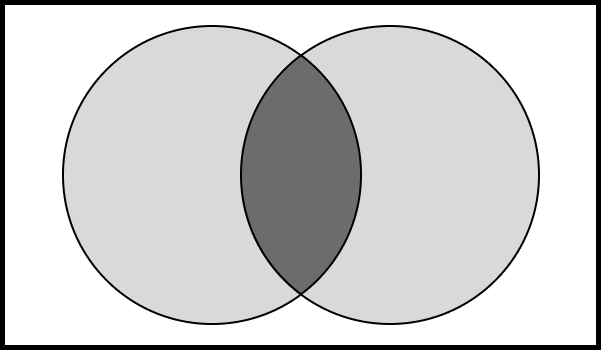
\includegraphics[width=0.25\textwidth]{tex/chapter_2/assets/Intersection.png}\\
    \end{center}
\end{definition}

\begin{definition}[Объединение множеств]
    Объединением множеств $A$ и $B$ называется множество, обозначаемое как $A \cup B$, состоящее из тех и только тех элементов, 
    которые принадлежат хотя бы одному из двух множеств. \\ 

    $A \cup B = \left\{ x \mid x \in A \lor x \in B \right\}$

    \begin{center}
        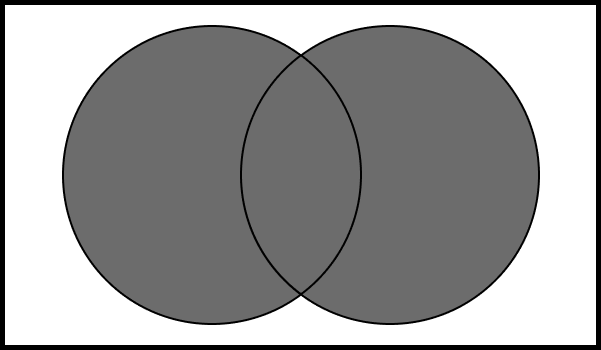
\includegraphics[width=0.25\textwidth]{tex/chapter_2/assets/Union.png}\\
    \end{center}
\end{definition}

\begin{definition}[Теоретико-множественная разность]
    Теоретико-множественной разностью множеств $A$ и $B$ называется множество, обозначаемое как $A \backslash B$, состоящее из тех и только тех элементов 
    множества $A$, которые не принадлежат множеству $B$. \\ 

    $A \backslash B = \left\{ x \mid x \in A \land x \notin B \right\}$

    \begin{center}
        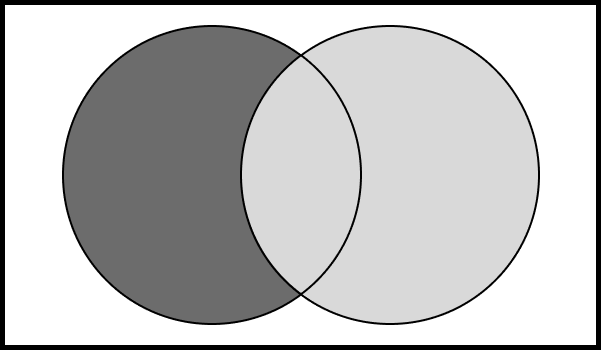
\includegraphics[width=0.25\textwidth]{tex/chapter_2/assets/Subtraction.png}\\
    \end{center}
\end{definition}
\section{Свойства теоретико-множественных операций}

\begin{theorem}[Коммуникативность пересечения]
    $A \cap B = B \cap A$
\end{theorem}

\begin{proof}
    Воспользуемся теоремами математической логики из модуля \ref{subsec:1.2.1} и определением пересечения

    \begin{align*}
        & \sphericalangle \; x \in A \cap B \leftrightarrow \\
        & x \in A \land x \in B \leftrightarrow \\
        & x \in B \land x \in A \leftrightarrow \\
        & x \in B \cap A \\
    \end{align*}
\end{proof}

\begin{theorem}[Ассоциативность пересечения]
    $A \cap (B \cap C) = (A \cap B) \cap C$
\end{theorem}

\begin{proof}
    Воспользуемся теоремами математической логики из модуля \ref{subsec:1.2.1} и определением пересечения

    \begin{align*}
        & \sphericalangle \; x \in A \cap (B \cap C) \leftrightarrow \\
        & x \in A \land x \in B \cap C \leftrightarrow \\
        & x \in A \land x \in B \land x \in C \leftrightarrow \\
        & (x \in A \land x \in B) \land x \in C \leftrightarrow \\
        & x \in (A \cap B) \land x \in C \leftrightarrow \\
        & x \in (A \cap B) \cap C \\
    \end{align*}
\end{proof}

\begin{theorem}[Дистрибутивность пересечения относительно объединения]
    \hfill \break \break
    $A \cap (B \cup C) = (A \cap B) \cup (A \cap C)$
\end{theorem}

\begin{proof}
    Воспользуемся теоремами математической логики из модуля \ref{subsec:1.2.1} и определениями пересечения с объединением

    \begin{align*}
        & \sphericalangle \; x \in A \cap (B \cup C) \leftrightarrow \\
        & x \in A \land x \in B \cup C \leftrightarrow \\
        & x \in A \land (x \in B \lor x \in C) \leftrightarrow \\
        & (x \in A \land x \in B) \lor (x \in A \land x \in C) \leftrightarrow \\
        & (x \in A \cap B) \lor (x \in A \cap C) \leftrightarrow \\
        & x \in (A \cap B) \cup  (A \cap C) \\
    \end{align*}
\end{proof}

\newpage

\begin{theorem}[Вычитание пересечения]
    $A \backslash (B \cap C) = (A \backslash B) \cup (A \backslash C)$
\end{theorem}

\begin{proof}
    Воспользуемся теоремами математической логики из модуля \ref{subsec:1.2.1} и определениями вычитания с пересечением

    \begin{align*}
        & \sphericalangle \; x \in A \backslash (B \cap C) \leftrightarrow \\
        & x \in A \land x \notin B \cap C \leftrightarrow \\
        & x \in A \land \neg (x \in B \land x \in C) \leftrightarrow \\
        & x \in A \land (x \notin B \lor x \notin C) \leftrightarrow \\
        & (x \in A \land x \notin B) \lor (x \in A \land x \notin C) \leftrightarrow \\
        & (x \in A \backslash B) \lor (x \in A \backslash C) \leftrightarrow \\
        & x \in (A \backslash B) \cup (A \backslash C)
    \end{align*}
\end{proof}

\begin{theorem}[Коммуникативность объединения]
    $A \cup B = B \cup A$
\end{theorem}

\begin{proof}
    Воспользуемся теоремами математической логики из модуля \ref{subsec:1.2.1} и определением объединения

    \begin{align*}
        & \sphericalangle \; x \in A \cup B \leftrightarrow \\
        & x \in A \lor x \in B \leftrightarrow \\
        & x \in B \lor x \in A \leftrightarrow \\
        & x \in B \cup A \\
    \end{align*}
\end{proof}

\begin{theorem}[Ассоциативность объединения]
    $A \cup (B \cup C) = (A \cup B) \cup C$
\end{theorem}

\begin{proof}
    Воспользуемся теоремами математической логики из модуля \ref{subsec:1.2.1} и определением объединения

    \begin{align*}
        & \sphericalangle \; x \in A \cup (B \cup C) \leftrightarrow \\
        & x \in A \lor x \in B \cup C \leftrightarrow \\
        & x \in A \lor x \in B \lor x \in C \leftrightarrow \\
        & (x \in A \lor x \in B) \lor x \in C \leftrightarrow \\
        & x \in (A \cup B) \lor x \in C \leftrightarrow \\
        & x \in (A \cup B) \cup C \\
    \end{align*}
\end{proof}

\newpage

\begin{theorem}[Дистрибутивность объединения относительно пересечения]
    \hfill \break \break
    $A \cup (B \cap C) = (A \cup B) \cap (A \cup C)$
\end{theorem}

\begin{proof}
    Воспользуемся теоремами математической логики из модуля \ref{subsec:1.2.1} и определениями пересечения с объединением

    \begin{align*}
        & \sphericalangle \; x \in A \cup (B \cap C) \leftrightarrow \\
        & x \in A \lor x \in B \cap C \leftrightarrow \\
        & x \in A \lor (x \in B \land x \in C) \leftrightarrow \\
        & (x \in A \lor x \in B) \land (x \in A \lor x \in C) \leftrightarrow \\
        & (x \in A \cup B) \land (x \in A \cup C) \leftrightarrow \\
        & x \in (A \cup B) \cap  (A \cup C) \\
    \end{align*}
\end{proof}

\begin{theorem}[Вычитание объединения]
    $A \backslash (B \cup C) = (A \backslash B) \cap (A \backslash C)$
\end{theorem}

\begin{proof}
    Воспользуемся теоремами математической логики из модуля \ref{subsec:1.2.1} и определениями вычитания с объединением

    \begin{align*}
        & \sphericalangle \; x \in A \backslash (B \cup C) \leftrightarrow \\
        & x \in A \land x \notin B \cup C \leftrightarrow \\
        & x \in A \land \neg (x \in B \lor x \in C) \leftrightarrow \\
        & x \in A \land (x \notin B \land x \notin C) \leftrightarrow \\
        & x \in A \land x \notin B \land x \in A \land x \notin C \leftrightarrow \\
        & (x \in A \land x \notin B) \land (x \in A \land x \notin C) \leftrightarrow \\
        & (x \in A \backslash B) \land (x \in A \backslash C) \leftrightarrow \\
        & x \in (A \backslash B) \cap (A \backslash C)
    \end{align*}
\end{proof}

\begin{theorem}
    $A \cap A = A$
\end{theorem}

\begin{theorem}
    $A \cap \varnothing = \varnothing$
\end{theorem}

\begin{theorem}
    $A \backslash \varnothing = A$
\end{theorem}

\begin{theorem}
    $A \cup A = A$
\end{theorem}

\begin{theorem}
    $A \cup \varnothing = A$
\end{theorem}

\begin{theorem}
    $A \backslash A = \varnothing$
\end{theorem}

\newpage
\section{Мощность множеств}

\begin{definition}[Мощность множеств]
    Для конечного множества мощность - количество его элементов. Мощность множества $A$ обозначают как $|A|$ 
\end{definition}

\begin{theorem}
    $|A \cup B| = |A| + |B| - |A \cap B|$
\end{theorem}

\begin{theorem}
    $|A \cup B \cup C| = |A| + |B| + |C| - |A \cap B| - |A \cap C| - |B \cap C| + |A \cap B \cap C|$
\end{theorem}
	

\end{document}

